%!TeX program=xelatex
\documentclass[a4paper]{article}

\usepackage{amsmath}
\usepackage{amssymb}
\usepackage[margin=1in]{geometry}
\usepackage{xcolor}
\usepackage{graphicx}
\usepackage{algorithm2e}
\usepackage{hyperref}
\hypersetup{
    colorlinks,
    linkcolor={red!50!black},
    citecolor={blue!50!black},
    urlcolor={green!50!black}
}
\usepackage{subcaption}
\usepackage[numbers]{natbib}

\usepackage{fontspec}
\setmainfont[Ligatures=TeX]{Palatino Linotype}

\newcommand{\fig}{Figure }

\begin{document}
  {\Large\noindent  Machine Learning on the Radio Galaxy Zoo}\\

  {\large\noindent  Matthew Alger \hfill Supervisor: Cheng Soon Ong}\\

  {\large\noindent  June 3, 2016}\\

  \begin{abstract}
    I did something and it kinda worked
  \end{abstract}

  \section{Introduction}

    \subsection{Cross-identification of Active Galactic Nuclei and Host Galaxies}

      Radio surveys such as Faint Images of the Radio Sky at Twenty-Centimeters (FIRST) \cite{white97,becker95} and the Australian Telescope Large Area Survey (ATLAS) \cite{franzen15} are dominated by \emph{active galactic nuclei} (AGNs) \cite{banfield15}, radio emissions emitted from the centre of galaxies by supermassive black holes\cite{peterson97}. Galaxies containing an AGN are referred to as \emph{host galaxies}. These galaxies are found in infrared surveys such as the Wide-field Infrared Survey Explorer (WISE) \cite{wright10} and the SIRTF Wide-area Infrared Extragalactic survey (SWIRE) \cite{surace05,lonsdale03}.

      Astrophysicists are interested in the properties of both AGNs and their host galaxies, but to investigate either, the AGNs need to be matched to their host galaxies. This is called \emph{cross-identification}. Many AGNs are associated with \emph{compact radio sources}, where the radio emissions directly and simply overlap the host galaxy (\fig \ref{fig:compact-source}), and these AGNs are easy to cross-identify\cite{banfield15}. However, many AGNS are instead associated with \emph{complex radio sources}, where radio emissions can be large, sprawling, and not relate to the host galaxy in any simple way (\fig \ref{fig:complex-source}).

      \begin{figure}[!ht]
        \centering
          \begin{subfigure}{0.3\textwidth}
            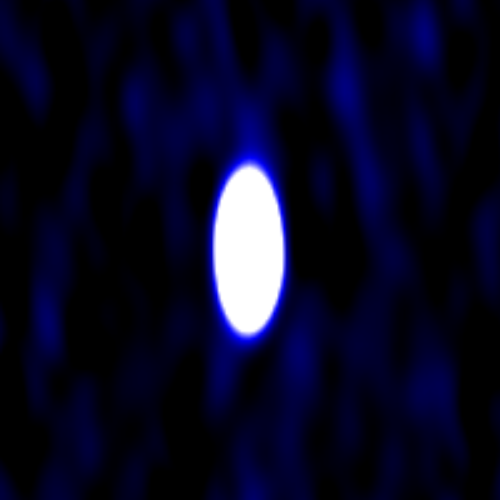
\includegraphics[width=\linewidth]{images/ARG0003r22_radio.png}
            \caption{A compact radio source.}
            \label{fig:compact-source}
          \end{subfigure}
          \quad
          \begin{subfigure}{0.3\textwidth}
            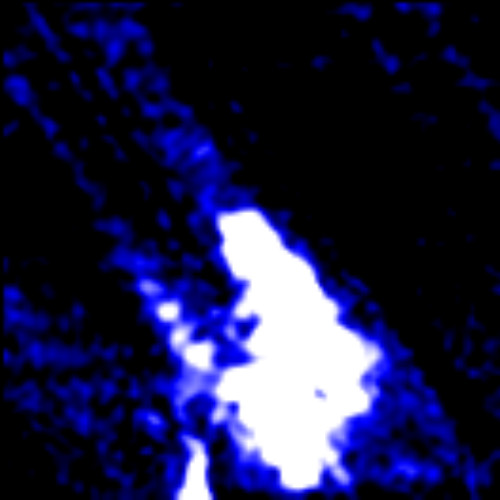
\includegraphics[width=\linewidth]{images/ARG0002dun_radio.jpg}
            \caption{A complex radio source.}
            \label{fig:complex-source}
          \end{subfigure}
          \caption{Example radio emissions.}
      \end{figure}

      \emph{Radio Galaxy Zoo}\footnote{\href{http://radio.galaxyzoo.org/}{Radio Galaxy Zoo}} is an online citizen science project that aims to crowdsource the cross-identification problem\cite{banfield15}. Volunteers are presented with a radio image of a small part of the sky (from FIRST or ATLAS) and the corresponding infrared image (from WISE or SWIRE). Each part of the sky presented in this way is called a \emph{subject}, and contains at least one radio emitter. Volunteers are asked to select which radio emissions are part of the same system, and which galaxy in the infrared image contains the corresponding AGN. The workflow is shown in \fig \ref{fig:rgz}.

      \begin{figure}[!ht]
        \centering
          \begin{subfigure}{0.3\textwidth}
            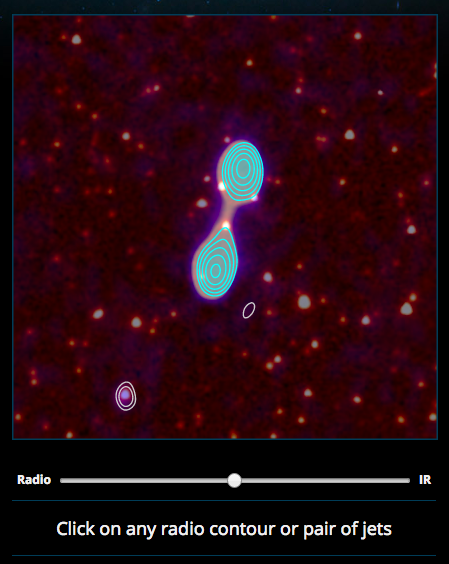
\includegraphics[width=\linewidth, height=2.3in]{images/rgz_radio.png}
            \caption{Select radio emissions.}
          \end{subfigure}
          \quad
          \begin{subfigure}{0.3\textwidth}
            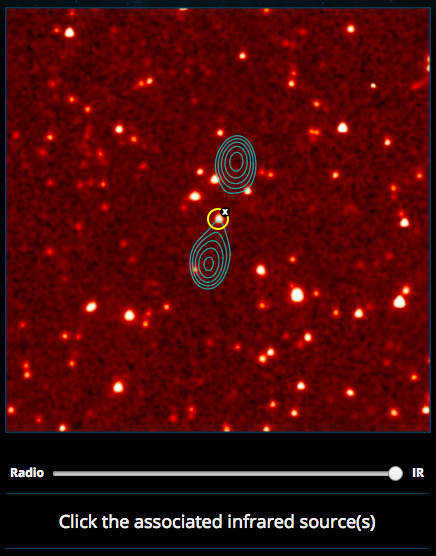
\includegraphics[width=\linewidth, height=2.3in]{images/rgz_ir.png}
            \caption{Locate the AGN.}
          \end{subfigure}
          \quad
          \begin{subfigure}{0.3\textwidth}
            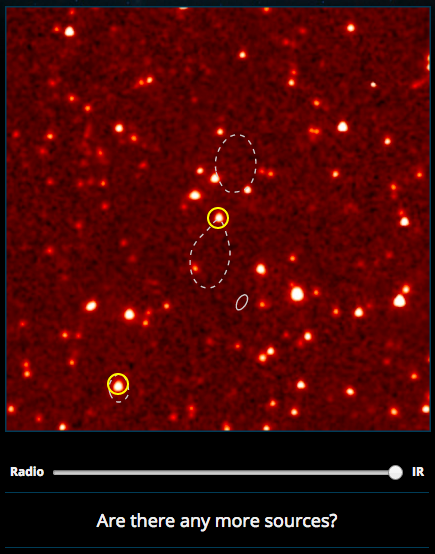
\includegraphics[width=\linewidth, height=2.3in]{images/rgz_done.png}
            \caption{Repeat for all emissions.}
          \end{subfigure}
          \caption{Radio Galaxy Zoo volunteer workflow.}
          \label{fig:rgz}
      \end{figure}

      Over 100000 radio sources have been classified by volunteers so far\footnote{Based on the data supplied to the author.} out of the Radio Galaxy Zoo database of around 177000 radio sources, compared to a few thousand classifications by experts\cite{banfield15}. However, new surveys such as the Evolutionary Map of the Universe (EMU) \cite{norris11} and Westerbork Observations of the Deep APERTIF Northern-Sky (WODAN) \cite{röttgering11} are expected to detect over 100 million radio sources\cite{banfield15}, making crowdsourcing an intractable solution to the cross-identification problem.

    \subsection{Related Work}

  \section{As Binary Classification}

  \section{A Pipeline}

  \bibliographystyle{abbrvnat}
  \bibliography{../papers}

\end{document}